\documentclass[10pt]{article}
\usepackage[margin=0.65in]{geometry}
\usepackage{mathptmx,graphicx,amsmath,hyperref}
\hypersetup{colorlinks=true,urlcolor=blue}
\pdfcompresslevel=9
\pdfobjcompresslevel=3
\setlength{\parindent}{0pt}
\setlength{\parskip}{5pt}
\begin{document}
\begin{center}
{\Large Candidate indices constrain RNG explanations}\\[3pt]
24 November 2026 --- source-data analysis
\end{center}
\textbf{Result.} The recorded indices contradict two complete families of
pure-visitation models: fixed extra draws after every candidate, and monotone
base-point retry costs after retained curves. These are conditional integer
arguments checked by a native reader of the existing 21 candidate and six
point-attempt observations. PCC-20261124-94d371 is producer-unverified.

\textbf{Assumptions.} Each candidate uses 20 successive calls; every visited
eligible candidate is retained. No hidden accepted output, restart, additional
filter, or unmodeled calls are allowed. Warmup may be arbitrary per field.
The post-retention model makes no extra calls after rejected candidates.

\textbf{1. Any fixed candidate cost.} With extra cost $d\geq0$, visited offsets
have spacing $20+d$, which must divide every published-offset difference.
P192 gives $\gcd(101780,15700)=20$; P239 gives
$\gcd(2700,14560)=20$. Thus $d=0$ in either field, leaving skipped eligible
indices between publications visited. No finite cost search is needed.

\textbf{2. Retry-driven post-retention cost.} After retained index$a$, an extra
cost$D$ must be divisible by 20 to reach the next published seed. Write $q=D/20$.
Missing skipped $s$ requires $q\geq s-a$; reaching the next retained $b$ requires
$q\leq b-a-1$. The recorded P239 gaps yield the incompatible ordering below.

\begin{center}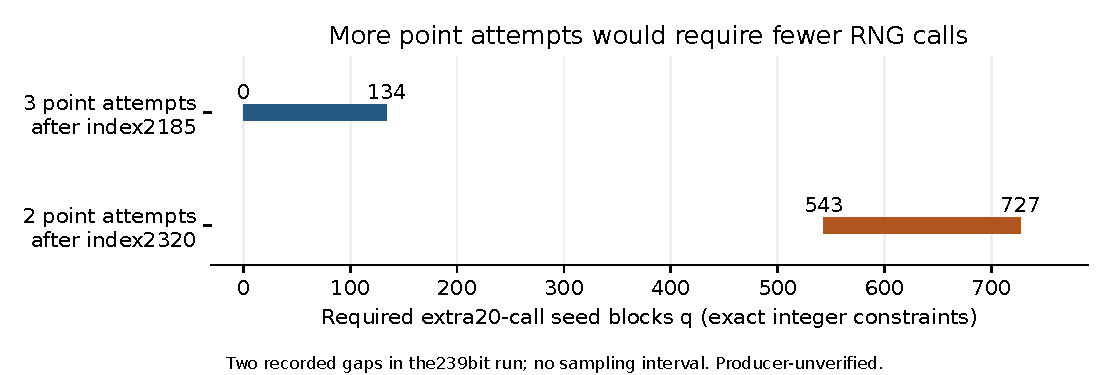
\includegraphics[width=.95\linewidth]{point-cost.pdf}\end{center}

The three-attempt event requires $D\leq2680$, while the two-attempt event
requires$D\geq10860$. No nondecreasing$D=f(r)$ satisfies these bounds.
P192 independently excludes$D=C+Lr$, $C,L\geq0$: its two-attempt event needs
$D_2\geq41180$, while its one-attempt event permits$D_1\leq15680$;
but$D_2\leq2D_1\leq31360$. A common initial burn also fails: P224 requires
at least 5736 seed blocks while P192 permits at most 138.

\textbf{Evidence and limits.} Native C++17 strict build and bounded integer
check exit 0; three positive/negative controls pass. First build indentation
errors and source are retained. All gap bounds are in
\texttt{evidence/constraints.tsv}; inputs and bytes are bound by the manifest.
No new curves, point counts, primality replay, RNG draws or paid job occurred.
Two producer checks are not independent signed verification. Lean/lake are
unavailable; no kernel-checked proof is claimed. The ordered-integer witnesses
are not polynomial identities over a finite field, so no identity-certificate
verdict is asserted. This does not explain all skips: calls after rejected
candidates or another independently specified caller path remain open.

\textbf{Sources.} Existing 21-row input table, crypto revision
\texttt{81f0308c75}, at\texttt{inputs/historical.tsv}.\\
Prior 52520-model search:\texttt{native/rng\_models.cpp}.
Point-attempt counts: \href{https://www.anthropic.com/research/ecdsa-curve-origins}{primary six-point reconstruction};
indices: \href{https://words.filippo.io/seeds-solved/}{independent enumeration}.
\end{document}
